% Kapittel 5 - Diskusjon
\chapter{Diskusjon}
\label{diskusjon} % Bruk \ref{diskusjon}, for å referere til kapittelet andre steder i oppgaven. 
%----------------------------------------------------------------------------------------
I dette kapittelet blir \textbf{de ulike beslutningene} som er tatt i løpet av utviklingen drøftet. \textbf{Forventinger og krav} som var satt til valgene og hva som ble de endelige avgjørelsene vil bli diskutert. I tillegg, inkluderer kapittelet diskusjon rundt \textbf{problemer med applikasjonen} og \textbf{forslag til forbedringer} ved videre utvikling.

\section{Begrunnelse og forklaringer knyttet til tekniske valg}
Det var flere tekniske valg som måtte tas før arbeidet med applikasjonen kunne starte. En av tankene i prosjektet var å \textbf{bruke metoder og hjelpemidler som er blant de mest aktuelle i dag}. Dette for å få nytte av god og oppdatert dokumentasjon, samt at produktet som utvikles skal bli \textbf{moderne og fremtidsrettet}.

\subsection{Hvorfor Angular ble valgt som web-rammeverk}
Det første og viktigste valget var hvilket \textbf{web-rammeverk} som skulle benyttes. På grunn av det store antallet JavaScript rammerverk/bibliotek som finnes i dag, var dette et krevende valg. I hovedsak var det tre rammeverk som ble vurdert: \textbf{React, Angular og Vue.js}. React og Angular er de to største, mens Vue.js har hatt en kraftig vekst de siste årene (figur \ref{fig:FrameworkPop}). I tillegg til disse tre, ble andre muligheter som \textbf{Ember.js og Backbone.js} også evaluert. Backbone.js ble utelatt fra vurderingen på grunn av alderen og oppdateringsfrekvensen. Backbone.js var et veldig populært rammeverk tidligere, men etter introduksjonen av moderne rammeverk har interessen dalt kraftig (figur \ref{fig:FrameworkPop}). Ember.js ble heller ikke vurdert videre da populariteten ikke kan sammenlignes med Angular/React og veksten ikke kan sammenlignes med Vue.js (figur \ref{fig:FrameworkPop}) \cite{jsFrameworks}.

\begin{figure}[H]
    \centering
    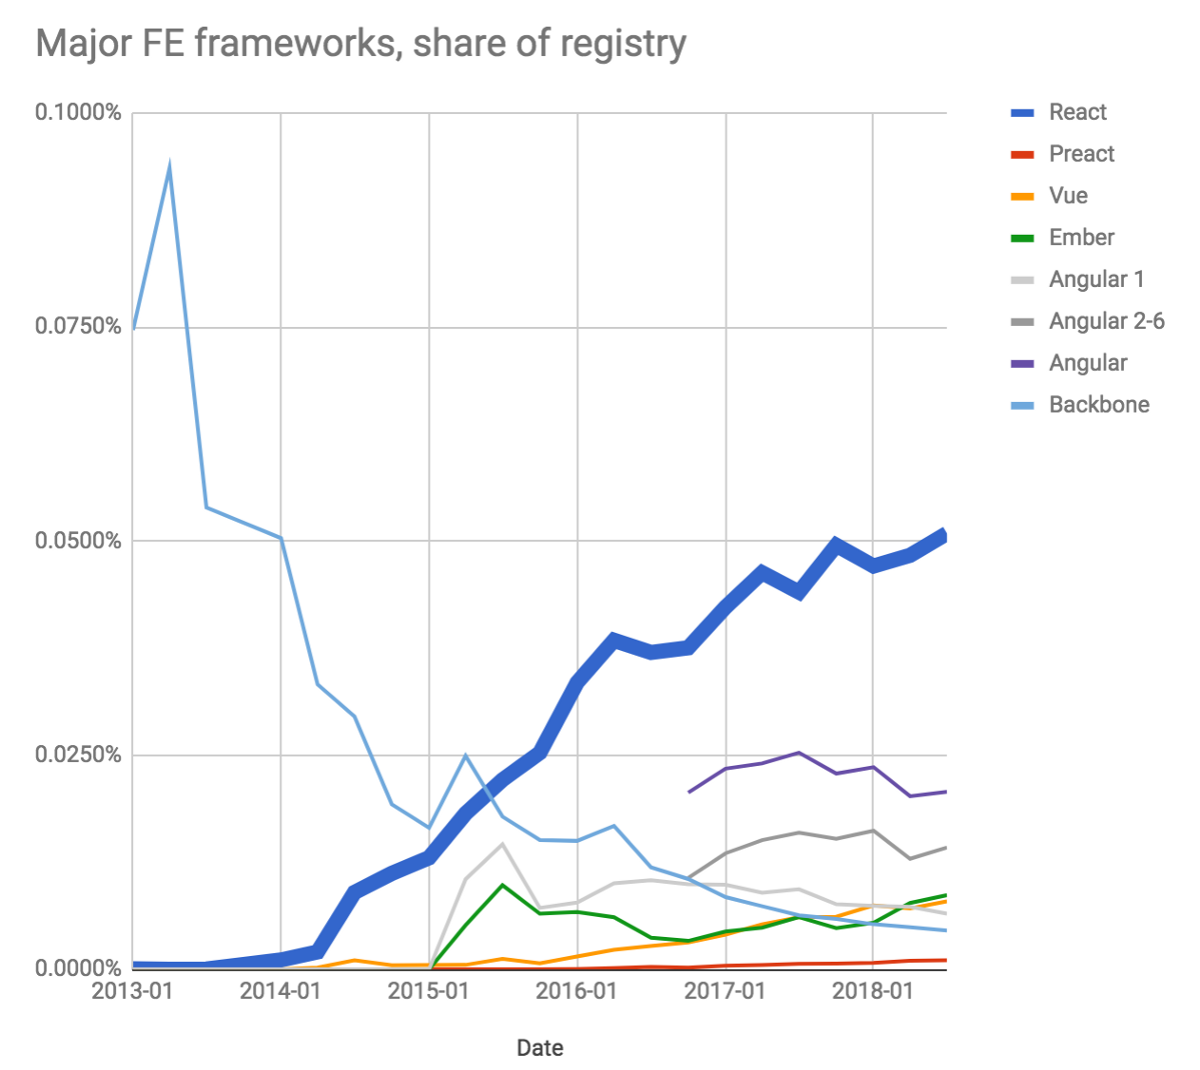
\includegraphics[width=0.9\textwidth]{Figurer/5Diskusjon/FEFrameworksShare.png}
    \caption{Frontend-rammeverk popularitet: andel av NPM-registeret \cite{jsFrameworks}}
    \label{fig:FrameworkPop}
\end{figure}

Alle tre frontend rammeverkene/bibliotekene, React, Angular og Vue.js, er \textbf{komponentbaserte} (beskrevet i kapittel \ref{AngularKomponenter}). Allikevel har de mange \textbf{ulike egenskaper} som gjør hver av dem mer/mindre egnet til ulike prosjekter.
\begin{itemize}
    \item \textbf{React} er et \textbf{JavaScript-bibliotek} for å bygge brukergrensesnitt \cite{reactHistory}. React ble opprinnelig laget av Facebook, men har i dag blitt åpen kildekode og vedlikeholdes av individuelle utviklere i tillegg til Facebook \cite{reactGithub}. En av egenskapene som skiller React fra andre bibliotek/rammeverk er syntaksen som består av en \textbf{blanding av \href{https://reactjs.org/docs/introducing-jsx.html}{JSX} og JavaScript}. I tillegg er React-applikasjoner basert på en \textbf{virtuell Document Object Model (DOM)}. En representasjon av brukergrensesnittet er lagret i minnet som synkroniseres med den «ekte» DOM-en. Dette gjør utvikling av applikasjoner enklere fordi React tar seg av attributt- og  hendelses-håndteringen samt DOM-oppdateringen. Dette måtte utvikleren ellers gjort selv \cite{reactVirtualDOM}. Det er også mulig med \textbf{enveis binding av data} i React. Dette binder variabler til HTML DOM-elementer og resulterer i at visningen (HTML) oppdateres automatisk hvis dataobjektet i programminnet (JS) oppdateres.
    
    \item \textbf{Angular} er et \textbf{fullverdig JavaScript-rammeverk} utviklet av Google og er etterfølgeren til Angular.js. Ettersom rammeverkene er svært forskjellige, er det viktig at de ikke forveksles med hverandre. I motsetning til de andre verktøyene bruker Angular \textbf{TypeScript som utviklingsspråk}. TypesScript er en Javascript-utvidelse som introduserer \textbf{statisk typing} og kan derfor gjøre det enklere å unngå bugs i utviklingsfasen \cite{staticTyping}. En annen unik egenskap med Angular, er muligheten for \textbf{toveis databinding}. Dette gjør det mulig å binde HTML DOM-elementer til objekter i programdata-en. Brukere kan da manipulere dataen som blir lagret \cite{AngularInformation}. Eksempelvis er dette brukt i brush-tabellen i programmet. Når brukeren endrer verdien i inputfeltene i tabellen, blir dette oppdatert umiddelbart og lagret i programminnet.
    
    \item \textbf{Vue.js} er i likhet med React et \textbf{Javascript-bibliotek} og ikke et rammeverk. Målet til grunnleggeren av Vue.js var å lage et \textbf{lett anvendelig bibliotek}. Dette ble realisert ved å la kjernen i Vue.js kun \textbf{fokusere på visningslaget} av applikasjonen. Kjernen kan utvides ved å legge til offisielle tilleggsbibliotek ved behov. Denne tilpasningsmuligheten beskrives ofte som Vue.js sin største fordel i forhold til Angular og React. Vue.js har, i likhet med React, kun \textbf{enveis data binding} \cite{VueInformation}.
\end{itemize}

\noindent Figur \ref{fig:FrameworkPop} viser at \textbf{Vue.js har hatt en bra vekst} de siste årene, men at \textbf{Angular og React er de mest populære}. Det ble derfor etter hvert besluttet å utelukke Vue.js fra den videre vurderingen. Deretter ble introduksjons-guidene til Angular og React gjennomført, for å få et bedre innblikk i hvordan begge fungerer. Guidene inkluderte en rask introduksjon hvor målet var å lage en liten applikasjon. Disse var nyttige for å få et innblikk i hvordan Angular og React fungerte.

\textbf{Angular blir ofte betraktet som vanskeligere å lære}, på grunn av størrelsen på rammeverket. Det finnes flere innebygde funksjoner og tjenester i Angular som kan være vanskelig å sette seg inn i med en gang \cite{angularvsreact}. 

For utviklere som kommer fra en objektorientert bakgrunn, med lite JavaScript-erfaring med JavaScript, kan Angular allikevel være lettere å lære seg enn React. TypeScript-implementasjonen gjør at \textbf{Angular har mer til felles med et standard objektorientert språk} som Java, C++ eller C\#.

Den endelige \textbf{beslutningen ble å bruke Angular som web-rammeverk} i dette prosjektet. \textbf{Funksjonene, støtten for TypeScript og mulighetene som er bygget inn i rammeverket} gjorde at Angular ble det foretrukne valget, til tross for React sin  som har en høyere popularitet.

\subsection{Hvorfor Chart.js ble valgt som graf-rammeverk}
En viktig del av denne applikasjonen er grafen som \textbf{viser frem informasjon om valgt brush}. En viktig beslutning i prosjektet var derfor å velge et passende graf-bibliotek. 

Biblioteket måtte ha mulighet til å \textbf{vise frem grafen på en oversiktlig måte, med et moderne utseende}. Målet ble derfor å finne et bibliotek som var enkelt i bruk og samtidig tilfredsstilte dette kravet. Det var kun ett enkelt stolpediagram som skulle bli vist frem, og derfor var mange grafmuligheter innad i biblioteket ikke så viktig. Det ble også lagt stor vekt på at det skulle være \textbf{enkelt å integrere biblioteket med Angular}. Etter å ha undersøkt mange ulike alternativer var det til slutt to kandidater som skilte seg ut: \textbf{Chart.js og Chartist.js}. Begge bibliotekene er åpen kildekode og det finnes utvidelser som gjør det enkelt å integrere dem i en Angular-applikasjon. 

\begin{itemize}
    \item \textbf{Chart.js} fokuserer på å være enkelt og brukervennlig. Antall valgmuligheter er derfor mindre enn i mange andre bibliotek. Chart.js inneholder 8 ulike typer grafer, hvor stolpediagram er en av dem. Utseendet til grafene som lages ved hjelp av Chart.js er \textbf{moderne og størrelsen er responsiv}  \cite{chartjs}. Utvidelsen \textbf{\href{https://github.com/valor-software/ng2-charts}{Ng2-charts}} gjør det enkelt å bruke biblioteket i Angular. Chart.js kan, etter integreringen, brukes som en hvilken som helst annen intern komponent i applikasjonen.
    \item \textbf{Chartist.js} prioriterer også å være et enkelt bibliotek. Allikevel inneholder Chartist.js en del \textbf{flere muligheter og graftyper enn Chart.js}. \textbf{Utseendet er moderne og responsivt}, men annerledes enn Chart.js \cite{chartistjs}. I likhet med Chart.js finnes det en utvidelse, \textbf{\href{https://github.com/willsoto/ng-chartist}{Ng-chartist}}, som gjør det lett å integrere Chartist.js i Angular-applikasjonen.
\end{itemize}

\noindent Disse bibliotekene har mange likhetstrekk og begge er gode alternativer. Siden grafen i denne applikasjonen \textbf{ikke hadde behov for avanserte tilpasningsmuligheter, falt valget til slutt på Chart.js}. 

\subsection{Hvorfor Bootstrap ble valgt som stil-rammeverk}
I oppstarten av dette prosjekter stod valget mellom \textbf{Bootstrap, Foundation og Angular Material} som verktøyet for å stilsette applikasjonen. Bootstrap og Foundation ble tatt med i vurderingen som følge av at de er blant de mest populære i dag \cite{top5frontend}. Angular Material ble vurdert fordi det utvikles av det samme teamet som utvikler Angular. Det var allerede bestemt at web-rammeverket for applikasjonen skulle være Angular, og derfor var det naturlig å ta med Angular Material i vurderingen. Det ble satt opp noen egenskaper (viktige og mindre viktige) for de ulike rammeverkene:

%Da dette valget ble tatt var det allerede bestemt at web-rammeverket for applikasjonen skulle være Angular. Det førte til at Angular Material også ble tatt opp til vurdering, ettersom det er et verktøy fra den samme plattformen. Det ble satt opp noen egenskaper (viktige og mindre viktige) for de ulike rammeverkene:

% Tabellfarger, Grønn: 2ECC40, Rød: FF4136, Gul: FFDC00
\begin{table}[ht]
\centering
\resizebox{\textwidth}{!}{%
\begin{tabular}{|l|
>{\columncolor[HTML]{2ECC40}}c |
>{\columncolor[HTML]{2ECC40}}c |
>{\columncolor[HTML]{2ECC40}}c |c|}
\hline
\multicolumn{1}{|c|}{
\cellcolor[HTML]{FFFFFF}\textbf{Egenskaper}} & \cellcolor[HTML]{FFFFFF}\textbf{Bootstrap} & \cellcolor[HTML]{FFFFFF}\textbf{Foundation} & \cellcolor[HTML]{FFFFFF}\textbf{Angular Material} & \cellcolor[HTML]{FFFFFF}\textbf{Viktig} \\ \hline

Tidligere erfaring & Ja & 
\cellcolor[HTML]{FF4136}Nei & 
\cellcolor[HTML]{FF4136}Nei & \checkmark \\ \hline
Responsivt design & Ja & Ja & Ja & \checkmark \\ \hline

Støtte for de fleste plattformer & Ja & \cellcolor[HTML]{FF4136}Nei & Ja & \checkmark \\ \hline

God dokumentasjon* & {\color[HTML]{000000} Ja} & Ja & Ja &  \\ \hline
Brukervennlig* & Ja & Ja & Ja &  \\ \hline

Mest brukt & Ja & \cellcolor[HTML]{FF4136}Nei & \cellcolor[HTML]{FF4136}Nei &  \\ \hline

Basert på rutenettsystem & Ja & Ja & Ja &  \\ \hline

Direkte linkede klasser & \cellcolor[HTML]{FF4136}Nei & Ja & \cellcolor[HTML]{FF4136}Nei &  \\ \hline
\end{tabular}%
}
* Subjektiv vurdering
\end{table}

\noindent \textbf{Valget falt til slutt på Bootstrap} ettersom det var dette rammeverket som \textbf{oppfylte flest av de viktige egenskapene}. Ved aktiv bruk av klassene i Bootstrap på elementene i applikasjonen, har nettsiden fått et \textbf{moderne preg}. Bruken av rammeverket har for det meste fungert bra, sett bort i fra et \textbf{importeringsproblem ved bruk av tooltipene}. Dette førte til at \textbf{Angular Material} sitt tooltip-verktøy ble \textbf{brukt som erstatter} på de aktuelle elementene. 

Selv om det er mange fordeler med Bootstrap så finnes det spesielt én stor ulempe. Ved å ta i bruk det mest brukte rammeverket får man \textbf{ikke noe unikt design} på nettsiden. Dette hensynet ble ikke vektlagt i denne applikasjonen, ettersom \textbf{funksjonaliteten hadde en høyere prioritet enn et unikt design}. 

\subsection{Hvorfor Git ble valgt som versjonskontroll}
Versjonskontroll er essensielt når det kommer til applikasjonsutvikling. Det finnes flere såkalte Distribuerte Versjonskontrollsystemer (DVCS), slik som Git, Mercurial, SVN, Bazaar, Darcs, osv. \textbf{Et DVCS holder styr på forandringer i filer} slik at en kan gå tilbake til spesifikke versjoner av applikasjonen senere. Det gjør at det blir \textbf{lettere å samarbeide og holde kontroll på endringer}. Valget av DVCS sto mellom \textbf{Git og Mercurial} da disse er blant de mest brukte i dag. Noen av de \textbf{ønskede egenskapene} som ble brukt i valget var:

\begin{table}[H]
\centering
\begin{tabular}{|l|
>{\columncolor[HTML]{2ECC40}}c |
>{\columncolor[HTML]{FF4136}}c |c|}
\hline
\multicolumn{1}{|c|}{\textbf{Egenskaper}} & \multicolumn{1}{c|}{\cellcolor[HTML]{FFFFFF}\textbf{Git}} & \multicolumn{1}{c|}{\cellcolor[HTML]{FFFFFF}\textbf{Mercurial}} & \multicolumn{1}{c|}{\textbf{Viktig}} \\ \hline
Tidligere erfaring & Ja & Nei & \checkmark \\ \hline
Slette og endre navn på grener & Ja & Nei & \checkmark \\ \hline
God dokumentasjon* & \cellcolor[HTML]{FF4136}Nei & Nei &  \\ \hline
Brukervennlig* & Ja & \cellcolor[HTML]{2ECC40}Ja &  \\ \hline
Mest brukt \cite{topDistributedVersionControlSystems} & Ja & Nei &  \\ \hline
\end{tabular}
\\ * Subjektiv vurdering
\end{table}

\noindent Ettersom \textbf{Git oppfylte de viktigste egenskapene}, ble det valgt som prosjektets versjonskontrollsystem. Dette har fungert som forventet og 
har vært en viktig faktor for at en god arbeidsflyt har blitt opprettholdt.

\subsection{Hvordan Git ble brukt som versjonskontroll}
I dette prosjektet hadde man \textbf{to hovedgrener}: «Master» og «Dev». \textbf{Master-grenen inneholdt siste stabile versjon av applikasjonen} og ble oppdatert regelmessig (fra dev-grenen) gjennom hele perioden. \textbf{Dev-grenen ble brukt til å implementere ny funksjonalitet}, og dette førte til at den inneholdt funksjoner som ikke alltid var skikkelig testet. For å effektivisere bruken av versjonskontrollen, ble det ofte opprettet nye grener ut fra dev-grenen. Dette ble gjort slik at man kunne arbeide fritt, uten at det førte til problemer i dev-grenen. Etter at en ny funksjonalitet var fullført i den nye grenen, ble den slått sammen med dev igjen. Dersom det ble oppdaget underveis at den nye funksjonaliteten ikke ville fungere, ble denne grenen bare slettet uten at dette skapte problemer for resten av prosjektet.

I figur \ref{fig:workflow2} kan man se et \textbf{eksempel på en arbeidsflyt} med en Master-, Hotfix-, Release-, Dev-gren og to Feature-grener. 

\begin{figure}[H]
\centering
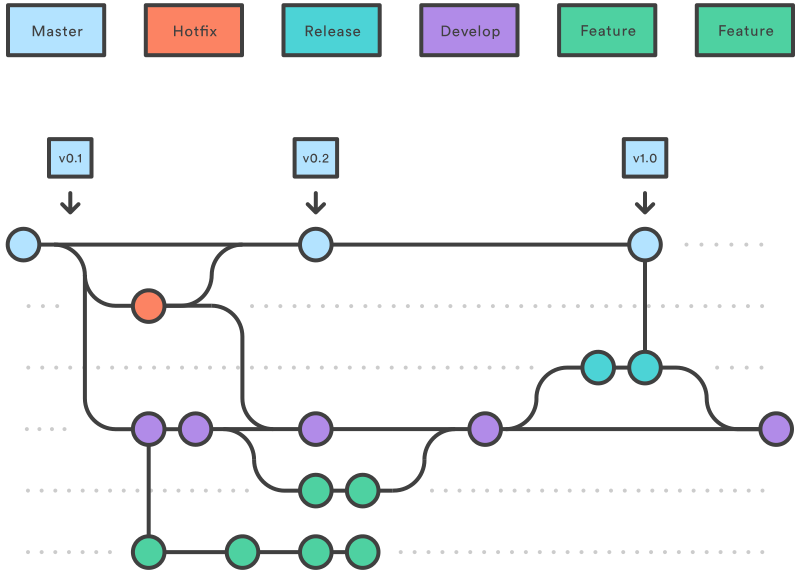
\includegraphics[width=0.9\textwidth]{Figurer/5Diskusjon/Workflow.png}
\caption{Eksempel på en workflow i Git \cite{workflow_bilde}.}
\label{fig:workflow2}
\end{figure}

\subsection{Hvorfor GitHub ble valgt som plattform}
Valget om hvilken plattform som skulle bli brukt for dette prosjektet stod mellom \textbf{GitLab og GitHub} (som følge av at Git ble valgt som versjonskontroll). Begge disse er \textbf{relativt like}. Blant annet støtter begge plattformene lagring av kildekode og andre filer i \textbf{oppbevaringsmapper}, slik at man får en bedre oversikt over prosjektet. For å kunne vurdere forskjellene mellom Github og Gitlab, ble det satt opp en liste med \textbf{avgjørende egenskaper}:
%Begge disse plattformene inkluderer støtte for å lagre kildekode og andre filer i oppbevaringsmapper slik at man får en bedre oversikt over prosjektet. Fordi GitHub og GitLab er \textbf{relativt like}, så det var vanskelig å finne avgjørende egenskaper:

\begin{table}[H]
\centering
\begin{tabular}{|l|
>{\columncolor[HTML]{2ECC40}}c |
>{\columncolor[HTML]{2ECC40}}c |c|}
\hline
\multicolumn{1}{|c|}{\textbf{Egenskaper}} & \multicolumn{1}{c|}{\cellcolor[HTML]{FFFFFF}\textbf{GitHub}} & \multicolumn{1}{c|}{\cellcolor[HTML]{FFFFFF}\textbf{GitLab}} & \multicolumn{1}{c|}{\textbf{Viktig}} \\ \hline
Tidligere erfaring & Ja & \cellcolor[HTML]{FF4136}Nei & \checkmark \\ \hline
Tilgang til fullversjon & Ja & Ja & \checkmark \\ \hline
Oppslagstavle med problemer & Ja & Ja & \checkmark \\ \hline
God dokumentasjon* & Ja & Ja &  \\ \hline
Enkel i bruk* & Ja & Ja &  \\ \hline
Private grener & Ja & Ja &  \\ \hline
Importering og eksportering av prosjekt & \cellcolor[HTML]{FF4136}Nei & Ja &  \\ \hline
Mest brukt \cite{top10versioncontrolsystems} & Ja & \cellcolor[HTML]{FF4136}Nei &  \\ \hline
\end{tabular}
\\ * Subjektiv vurdering
\end{table}

\noindent Den \textbf{tidligere erfaringen ble avgjørende} i dette valget og førte til at \textbf{GitHub ble valgt} som arbeidsplattform. GitHub har \textbf{flere nyttige funksjoner}, deriblant \textbf{«GitHub Issues»} hvor man kan holde oversikt over oppgaver, forbedringer og feil i prosjektet \cite{githubIssues}. Dette ble brukt som et verktøy hvor man raskt kunne \textbf{se hva som måtte gjøres}, og samtidig \textbf{se tilbake på ting som hadde blitt gjort}. Nye punkter ble lagt til etter hvert som prosjektet utviklet seg og markert ferdige når de var implementert. Figur \ref{fig:github_issues} viser en skjermdump fra GitHub Issues underveis i dette prosjektet.

\begin{figure}[H]
\centering
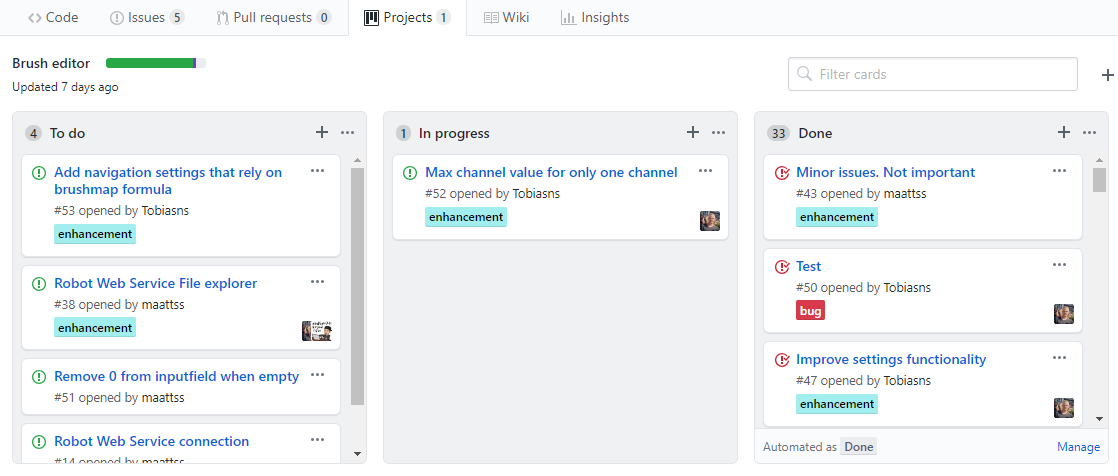
\includegraphics[width=0.9\textwidth]{Figurer/5Diskusjon/GitHub_issues.PNG}
\caption{GitHub Issues fra prosjektet (hentet 26.03.2019).}
\label{fig:github_issues}
\end{figure}

\section{Begrunnelse av designvalg}
I forbindelse med hvordan nettsiden skulle se ut og hva som skal fokuseres på, har det blitt tatt ulike designvalg i prosjektet. Hvordan dette har blitt gjort og hvorfor de ulike valgene har blitt tatt vil bli diskutert nærmere i dette delkapittelet.

\subsection{Hvorfor det var størst fokus på mobil}
De siste årene 10 årene har bruken av internett på håndholdte enheter eksplodert \cite{platformStats}. På grunn av dette har det i de senere årene blitt mer og mer vanlig å fokusere på et mobilvennlig brukergrensesnitt ved utvikling av nye webapplikasjoner. Dette har også vært tilfelle i dette prosjektet. Dagens løsning hos ABB er, som nevnt tidligere, en Windows-applikasjon. For å øke fleksibiliteten og gjøre det enklere for brukerne å redigere brush-filer, har fokuset helt fra starten av vært å utvikle et bra mobilt grensesnitt med et responsivt design. Målet har vært å kunne ha samme funksjonalitet som dagens løsning, i en oversiktlig webapplikasjon. Dermed kan brukerne stå fritt til å velge hvilkeen enhet de vil benytte seg av.

\subsection{Design og oppsett av komponentene}
Etter hvert som nye komponenter og funksjoner ble lagt til, var det viktig at disse også fikk en passende plasseringen i layouten. Det har derfor vært en del \textbf{endringer i det grunnleggende designet underveis i prosjektet}. Tidlig i utviklingen var det svært få komponenter å holde styr på, men etter hvert som flere har blitt lagt til har det vært viktigere å opprettholde strukturen. \textbf{Målet har vært å holde designet oversiktlig} slik at brukeren ikke må streve for å finne ut hvordan applikasjonen skal brukes. 

\begin{figure}[H]
\centering
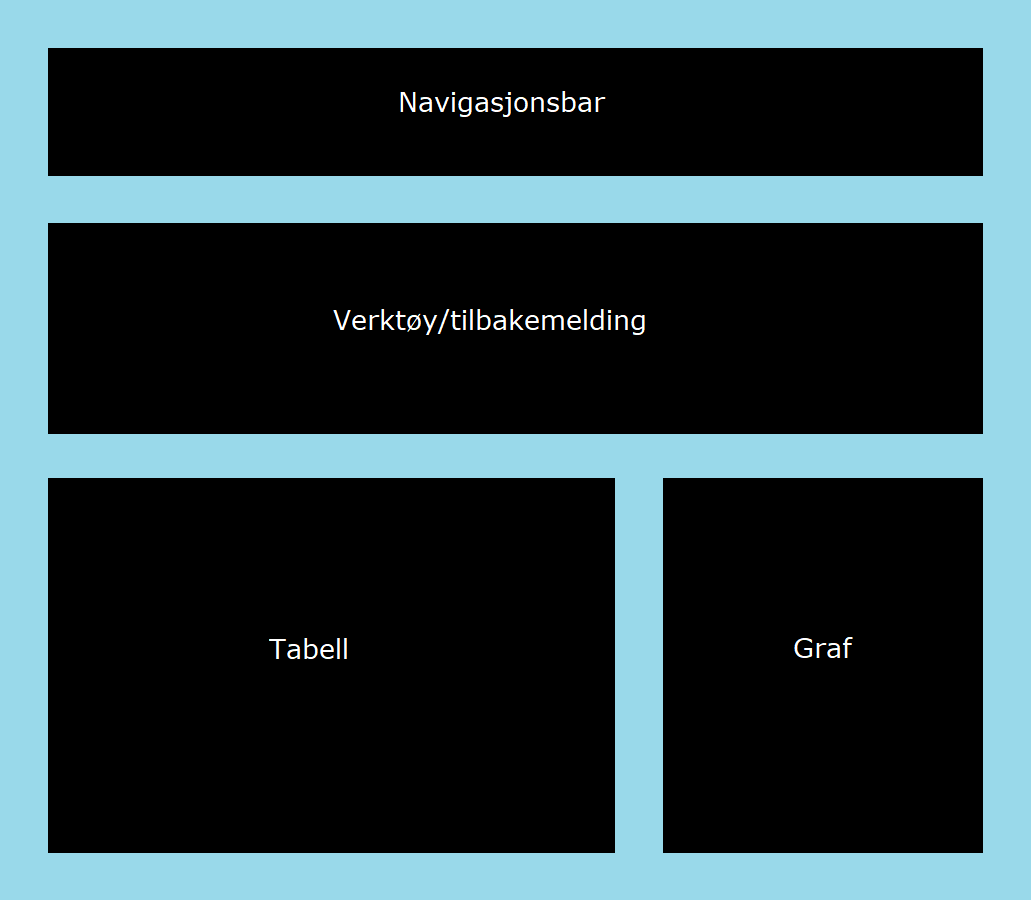
\includegraphics[width=0.9\textwidth]{Figurer/5Diskusjon/Komponenter.png}
\caption{Strukturen til komponentene i applikasjonen.}
\label{fig:komponenter}
\end{figure}

I feltet \textbf{«Navigasjonsbar»} befinner det seg en \textbf{liggende navigasjonsbar} som blir vist frem i toppen av vinduet til enhver tid. Denne er satt her for å gjøre det enkelt å åpne viktige verktøy. Hvis applikasjonen nettopp er åpnet vil dette være den eneste komponenten som viser frem noe. 

I feltet \textbf{«Verktøy/tilbakemelding»} vil det \textbf{variere hva som blir vist frem} og feltet vil fjernes dersom ingenting er valgt. Det som kan bli vist er her; \textbf{brush-mapping, robot-filutforsker, filinformasjon, innstillinger, feil- og suksessmeldinger}. Det kan \textbf{ikke bli vist frem flere av disse komponentene på samme tid} (foruten om feil- og suksessmeldinger, som er uavhengige). Vurderingen har vært at det ikke er nødvendig å vise disse komponentene samtidig og at dette kunne skapt \textbf{en uoversiktlig applikasjonen}. En \textbf{egen visningstjeneste er definert}. Denne inneholder funksjoner som holder styr på hvilke komponenter som skal åpnes/lukkes etter hvert som brukeren tar ulike valg.

I feltene \textbf{«Tabell»} og \textbf{«Graf»} vil \textbf{brush-tabellen og den tilhørende grafen vises}. Disse komponentene vil alltid bli vist så lenge en brush-fil er lastet inn. Grunnen til dette er at de er relevante for de fleste komponentene som befinner seg i «Verktøy/tilbakemelding»-feltet. \textbf{Dersom skjermen til brukeren er for liten} til å vise de to komponentene side om side, \textbf{vil grafen automatisk posisjonere seg under tabellen}. 

\begin{figure}[H]
    \centering
    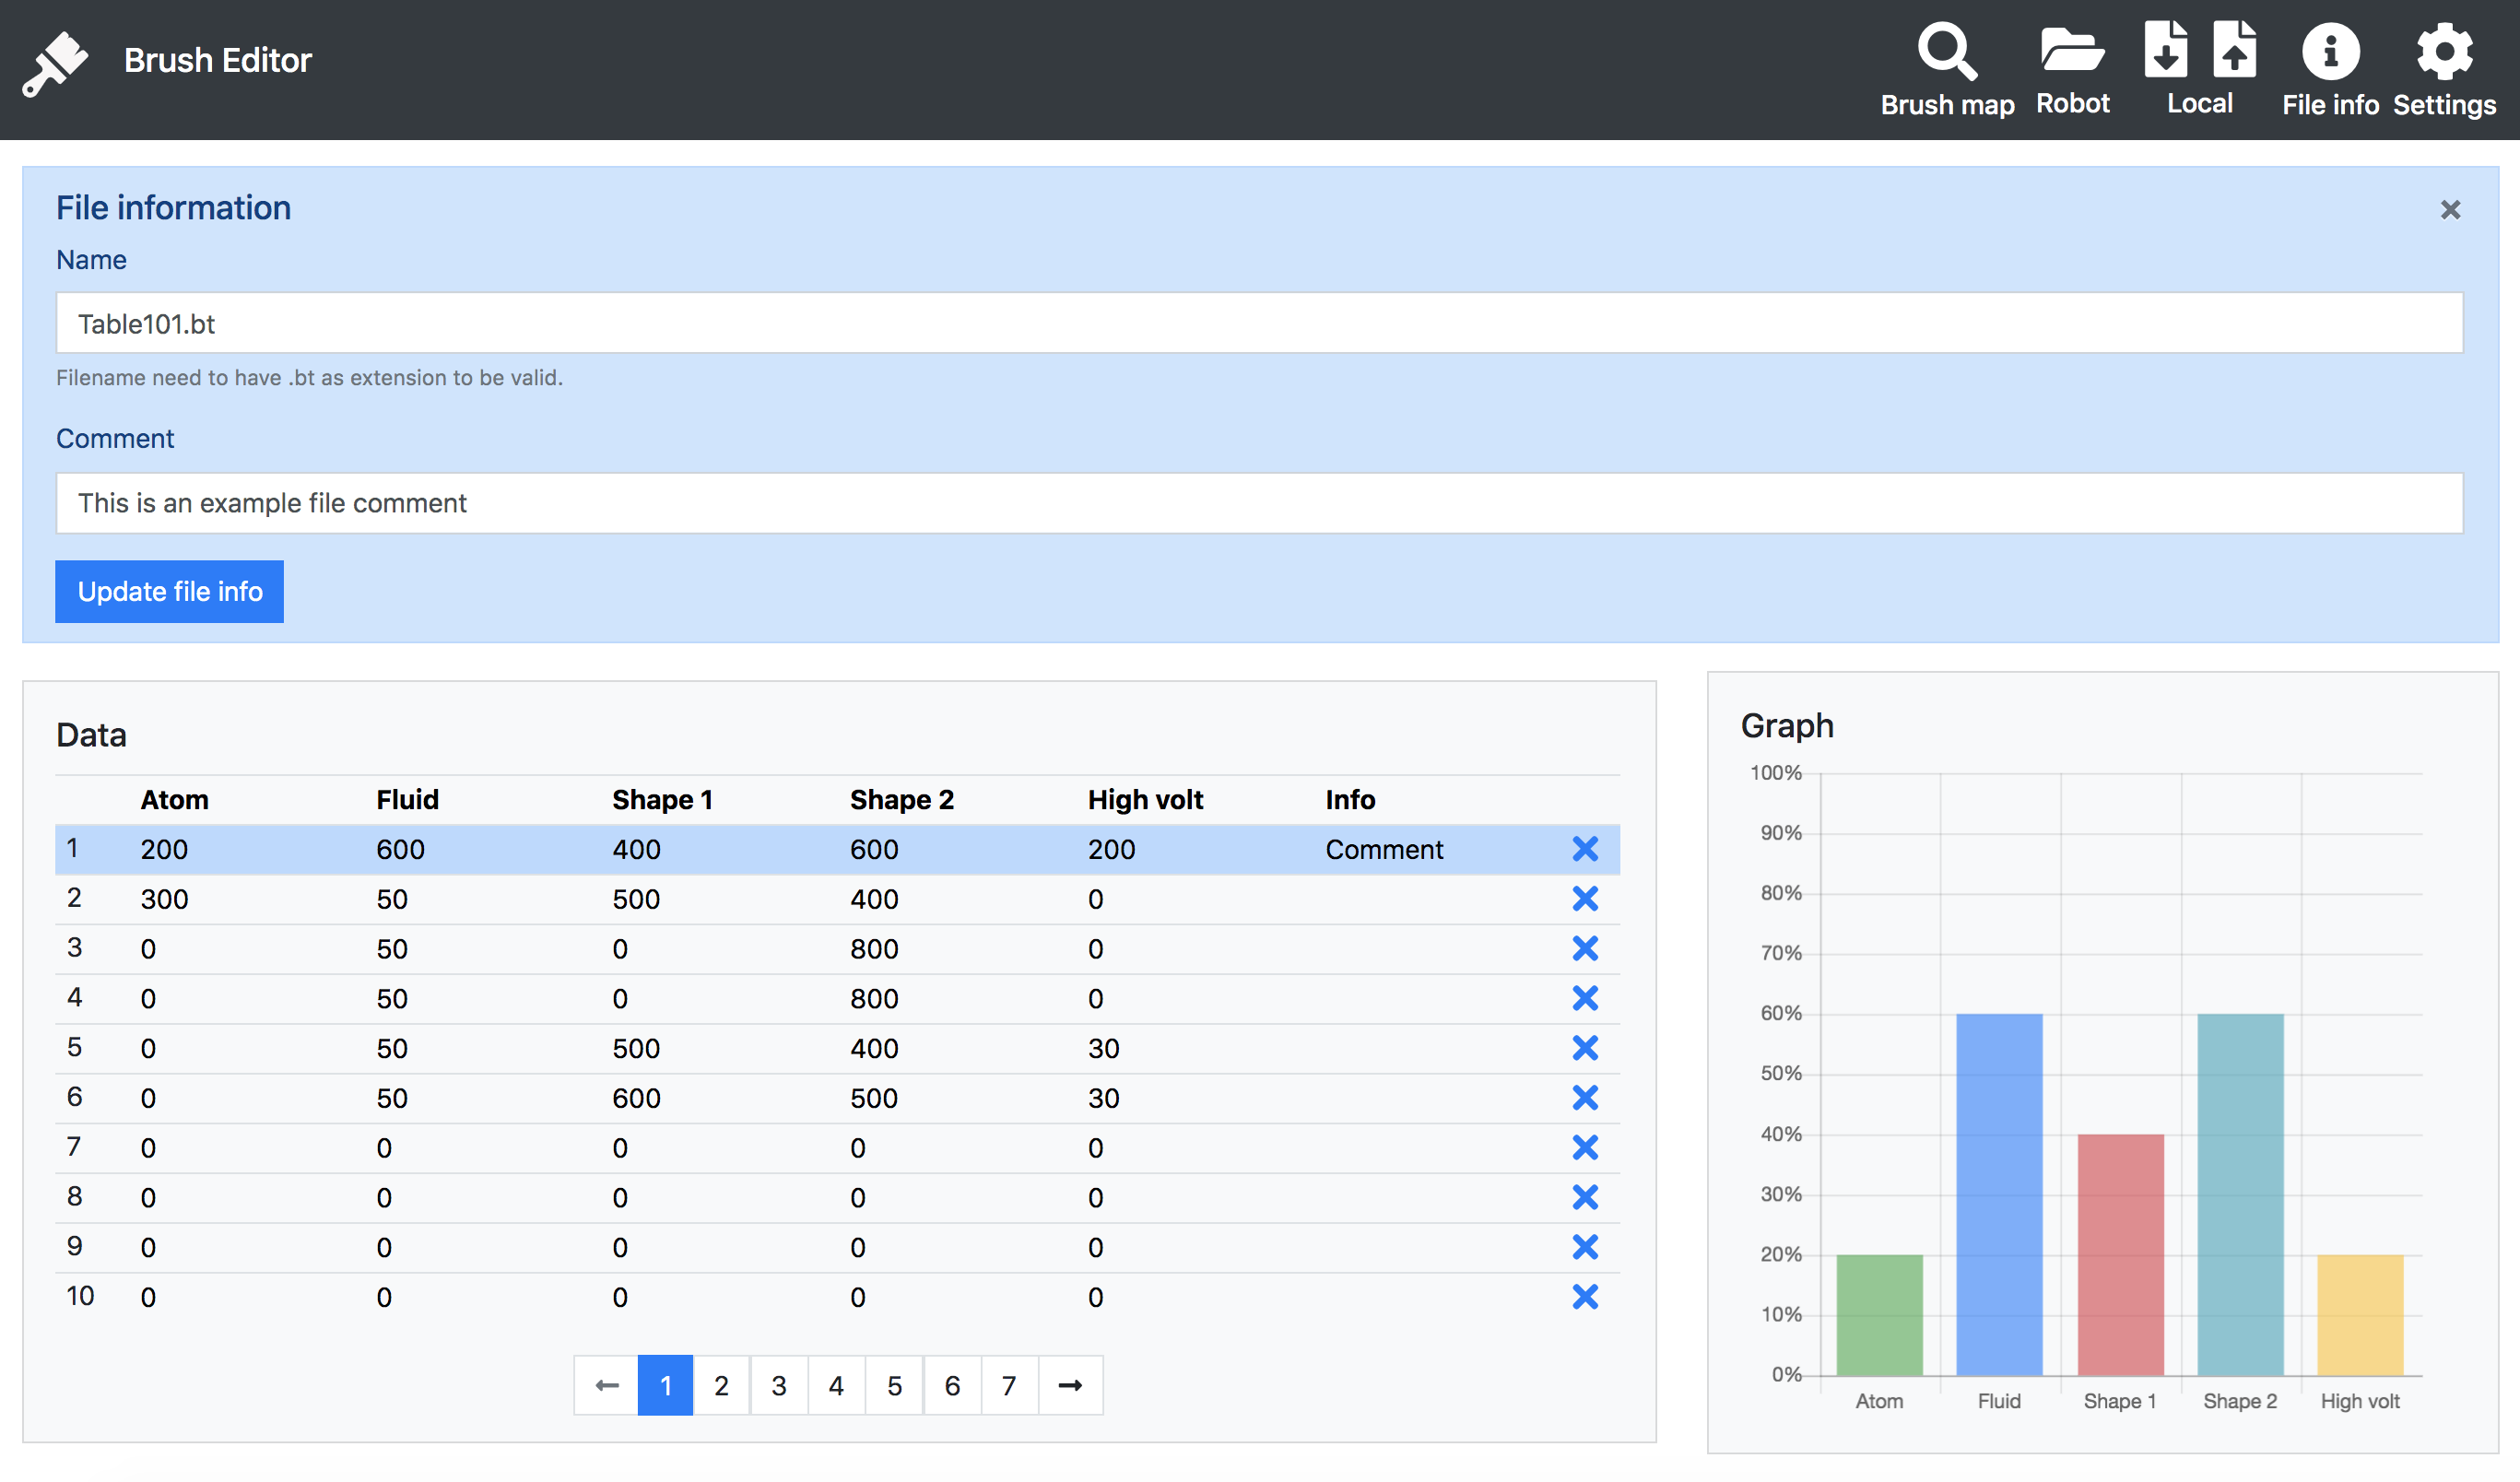
\includegraphics[width=0.9\textwidth]{Figurer/5Diskusjon/Oversikt.png}
    \caption{Oversiktsbilde av applikasjonen.}
    \label{fig:oversikt}
\end{figure}

\section{Tilbakemelding fra brukere av dagens løsning}
Denne applikasjonen har blitt \textbf{testet av ansatte i ABB} som har erfaring med det nåværende programmet. De ulike funksjonene i applikasjonen ble testet og det ble samlet inn tilbakemeldinger om \textbf{hva som var bra} og \textbf{hva som eventuelt kunne forbedres}. Noen av de punktene som gikk igjen er listet opp under:

\begin{itemize}
\item Mer informasjon til brukeren om hvor dataene som blir vist kommer fra og hva de representerer.
\item Flere innstillingsmuligheter slik at applikasjonen blir mer fleksibel.
\item Flere redigeringsmuligheter av brush-dataene i tabellen slik at man ikke måtte gjøre dette manuelt i brush-filene.
\end{itemize}

\noindent Tilbakemeldingene ble nyttige i diskusjonen av hva som bør prioriteres ved videre utvikling av applikasjonen.

\section{Forslag til forbedringer ved videre utvikling}
For å gjøre videreutvikling av denne applikasjonen lettere, blir det i dette delkapittelet tatt for seg ulike \textbf{forbedringspotensialer til applikasjonen}. Disse kan brukes til å ta applikasjonen ett steg videre. \textbf{Knapp tid} har i de fleste tilfellene vært den avgjørende faktoren for at disse forbedringene ikke har blitt gjennomført. 

\subsection{Mer informasjon til brukeren}
Et av de viktigste \textbf{forbedringspotensialene} (som også ble nevnt i tilbakemeldingene) er å \textbf{vise frem mer informasjon}. Selv om mye av informasjonen som er ønsket allerede finnes ulike steder i applikasjonen, hadde en forbedret visning av disse styrket programmet. \textbf{Noen eksempeler} på hvilken informasjon brukerne ville se tydeligere er:

\begin{itemize}
    \item \textbf{Hvilken robot applikasjonen er koblet til.} 
    \item Synligere \textbf{informasjon om kanalene} (maks kanalverdi, måleenhet, etc.).
    \item Informasjon om \textbf{filen som er åpen} i tabellen.
    \item Hvilken \textbf{versjon av applikasjonen} som er i bruk.
\end{itemize}

\noindent Dersom man går inn i \textbf{innstillingene} vil \textbf{IP-adressen} til den valgte roboten og informasjon om \textbf{maksverdi} (dersom man velger en kanal) \textbf{bli synliggjort}. Dersom brukeren \textbf{ikke har benyttet applikasjonen} før, kan det nok være \textbf{litt vanskelig å forstå} at man må åpne innstillingene for å få tilgang til denne informasjonen. Et \textbf{forslag} til løsning kan derfor være å \textbf{vise informasjon om den valgte roboten} over tabellen og lage \textbf{tooltips til kanalene} for å vise frem maksverdi, måleenheten og annen nødvendig informasjon. 

Man finner også informasjon om \textbf{hvilken fil som er åpen} i tabellen dersom man åpner filinformasjonen. \textbf{Filinformasjonskomponenten trengs} ettersom den gir rom for å \textbf{endre} på både \textbf{filnavn og -kommentar}. Det kunne likevel blitt \textbf{vist frem filnavn} over tabellen slik at brukeren \textbf{ikke trenger} å åpne filinformasjonskomponenten for å få tak i denne informasjonen. Her kunne også \textbf{versjonsnummeret} til applikasjonen blitt vist frem.

\subsection{Flere redigeringsmuligheter til brush-dataene i tabellen}
Den eneste \textbf{nåværende redigeringsmuligheten} i applikasjonen er å \textbf{slette innholdet i en rad} (sette alle verdiene til 0). Den ble lagt til slik at brukeren slipper å gjøre dette manuelt, for alle verdier i raden, dersom det er nødvendig. Det kunne med fordel vært \textbf{lagt til flere} redigeringsvalg som:

\begin{itemize}
\item Legge til/fjerne rader i tabellen. 
\item Tillate innskriving av ugyldige verdier i tabell, men vis at det ikke er mulig å lagre disse verdiene.
\end{itemize}

\noindent \textbf{Legge til og fjerne rader} er noe som i dag må gjøres \textbf{manuelt} i brushfilen. Dette er en \textbf{tungvint løsning} og det kunne derfor vært nyttig å \textbf{legge til dette} som en mulighet i applikasjonen.
For eksempel, kunne dette blitt gjort ved å legge til en \textbf{ny knapp} i hver rad, som \textbf{fjerner hele raden}. I tillegg til en knapp under nederste rad i tabellen som \textbf{legger til en ny}.

%Det kunne for eksempel blitt \textbf{lagt til mulighet for å fjerne hele raden} ved en knapp på enden av den aktuelle raden og så kunne det blitt lagt til en knapp under nederste rad i tabellen der man kunne \textbf{lagt til en rad}.


I denne applikasjonen er det brukt \textbf{inputvalidering} for å sørge for at brukeren ikke har muligheten til å taste inn \textbf{ugyldige verdier}. En forbedring her (ifølge tilbakemeldingene) kunne vært å \textbf{la brukeren taste inn ugyldige verdier}, men la de få en form for \textbf{beskjed om at verdien er ugyldig}. Dette var ønskelig ettersom \textbf{brukerne som regel har god kontroll} på hvilke verdier som er ugyldige, men at de vil \textbf{oppbevare dem der midlertidig}.

\subsection{Flere innstillinger i applikasjonen}
Det finnes  \textbf{tre ulike innstillingsmuligheter} i denne applikasjonen. Det er mulig å  \textbf{endre maksverdi} for en kanal, \textbf{endre IP-adresse} for å bytte robot og  \textbf{tilbakestille kanalnavn} til standard. Det kunne fint vært lagt til  \textbf{flere innstillingsmuligheter} enn de som eksisterer. Noen  \textbf{forslag} som kom frem fra tilbakemeldingene var:

\begin{itemize}
\item Mulighet til å  \textbf{endre utseendet} til applikasjonen.
\item Mulighet til å \textbf{endre språk}. 
\end{itemize} 

Ved  \textbf{endring av utseendet} kunne det for eksempel blitt lagt til mulighet for å  \textbf{endre farge på søyler i grafen}, introdusert et valg for  \textbf{ «mørk modus»}, etc. Angående mulighet til å  \textbf{endre språk} kunne man hatt et  \textbf{engelsk og norsk} flagg ved siden av hverandre oppe i et hjørne, slik at brukeren kunne valgt  \textbf{hvilket språk som skulle bli brukt}. Ellers er det lurt å tenke over uttrykket  \textbf{ «less is more»} og ikke legge til innstillinger som  \textbf{ikke har en nytteverdi} for brukerene. Dette vil  \textbf{føre til} en mer  \textbf{uoversiktlig} applikasjon. 


Det finnes tre ulike innstillingsmuligheter i denne applikasjonen:

\begin{itemize}
\item Endre maksverdi for en kanal.
\item Endre IP-adresse for å bytte robot.
\item Tilbakestille kanalnavn til standard.
\end{itemize}

\noindent Et klart forbedringspotensiale er inkludering av flere innstillingsmuligheter. Et forslag her (fra tilbakemeldingene) var å legge til muligheten til å ender utseendet til applikasjonen. Dette kan være i form av farge på søylene i grafen, eller introduksjon av valg for «mørk modus».
 
Forøvrig er det lurt å tenke over uttrykket «less is more» og ikke legge til innstillinger som ikke har en nytteverdi for brukerene. Dette vil kunne føre til en mer uoversiktlige applikasjon.

\subsection{Flere funksjoner i filvelgeren}
Komponenten hvor man har muligheten til å \textbf{åpne og bla i filer fra filsystemet til robotkontrolleren} kunne vært \textbf{utvidet med flere funksjoner}. Per dags dato er det kun mulig å bla gjennom filstrukturen, åpne filer i Brush Editoren og eksportere åpnet fil. Robot Web Service REST API inneholder flere muligheter som kunne vært nyttige å inkludere i filvelgeren:

\begin{itemize}
    \item \textbf{Opprette ny mappe/fil}
    \item \textbf{Slette mappe/fil}
    \item \textbf{Endre navn på mappe/fil}
    \item \textbf{Duplisere mappe/fil}
\end{itemize}

\noindent Dette er \textbf{ikke kritiske funksjoner}, men de hadde gjort filvelgeren mer komplett. Målet med dette prosjektet er på sikt å kunne bytte ut den eksisterende Windows-applikasjonen og det er da en fordel at slike funksjoner er på plass. Mulighetene ligger, som sagt, allerede i REST API-et, så det er ingen tekniske utfordringer knyttet til implementasjonen. \textbf{Knapp tid} var det som gjorde at disse funksjonene ble nedprioritert i dette prosjektet.

\subsection{Sikrere autentiseringsmetode enn Digest}
Det er brukt Digest for å autentisere brukere som skal koble seg opp til Robot Web Service (API). I dag vurderes denne formen for autentisering ofte som \textbf{mindre sikker}. Selv om Digest er sikrere enn Basic Authentication (forklart i kapittel \ref{basicAuthentication}), har metoden likevel klare mangler:

\begin{itemize}
\item \textbf{Krypteringen (MD5) er utdatert og reversibel} \cite{md5_outdated}. Det resultere i at angripere kan få tak i brukernavn og passord til brukere.
\item Det er \textbf{til en viss grad sårbart for replay-angrep}: En person kan klare å snappe opp det hashede passordet for å få tilgang til de passordbeskyttede ressursene, illustrert i figur \ref{fig:replayAttack}. Selv om det blir brukt en engangsverdi (nonce) for hver tilkobling, så er det opp til serveren å sjekke at engangsverdien ikke blir brukt flere ganger. Hvis dette ikke blir sjekket av serveren, vil det være mulig å utføre et replay-angrep \cite{replayAttack}.
\end{itemize}

\begin{figure}[H]
\centering
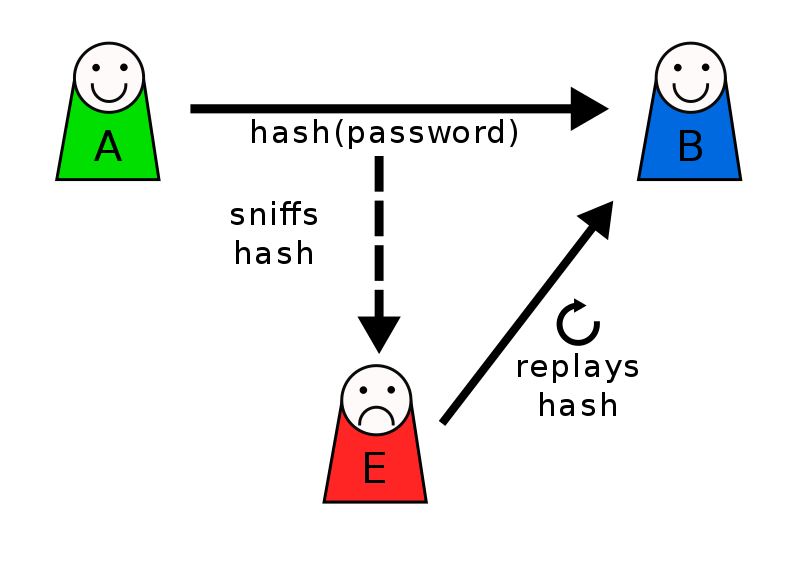
\includegraphics[width=0.9\textwidth]{Figurer/5Diskusjon/Replay_attacks.png}
\caption{Eksempel på hvordan et replay-angrep fungerer \cite{replay_attack_bilde}.}
\label{fig:replayAttack}
\end{figure}

\noindent For å forbedre sikkerheten kunne en mulig løsning vært å \textbf{bytte til en mer moderne autentiseringsmetode}, for eksempel OAuth 2.0 (forklart i kap \ref{OAuth}). Det finnes flere fordeler med å bruke OAuth istedenfor Digest. Her er noen av dem:
\begin{itemize}
\item \textbf{Brukernavn og passord blir ikke sendt mellom klient og server} slik som i Digest. Det vil istedenfor bli brukt en autentiseringskode (token) for å autentisere brukeren. Denne autentiseringskoden inneholder ingen brukernavn eller passord og vil utløpe etter kort tid. 
\item \textbf{Ulike adgangsnivåer}: read-only eller read-write. Det vil si at man kan velge om brukeren skal kun skal ha mulighet til å hente filer eller om det også skal bli gitt tilgang til å overskrive filer fra roboten.
\item Man kan \textbf{velge hvilken informasjon som skal være tilgjengelig/skjult} for brukeren.
\end{itemize}

\noindent Ulempen er at det er \textbf{krevende å sette opp OAuth}, men dette ville hevet sikkerheten i kommunikasjonen mellom robotkontrolleren og applikasjonen betydelig.

\subsection{Forbedre kodestrukturen}
Koden i dette prosjektet har, som i de fleste prosjekter, rom for forbedring. En av de største er: \textbf{Mer bruk av Angular sine egne moduler}. Disse modulene inneholder flere funksjoner som forenkler utviklingsprosessen betraktelig. 

En ryddig kodestruktur er en av hovedfordelene ved å implementere ferdige moduler. I tillegg minker sjansen for å gjøre noe som frembringer feil i applikasjonen. Problemet med modulene er at det kan være \textbf{komplisert og tidkrevende å sette seg inn i} dem. Derfor kan det være lurt å bare bruke Angular sine ferdige moduler ved implementasjon av store og kompliserte funksjoner. Dette er noe som må vurderes i hvert enkelt tilfelle. 

I denne applikasjonen er det i hovedsak \textbf{to moduler som kunne blitt brukt/brukt mer} i applikasjonen: 

\begin{itemize}
    \item \textbf{Angular Router} er Angular sin ruting-tjeneste. Denne tar hånd om å \textbf{navigere brukeren mellom forskjellig visninger i applikasjonen} \cite{angularRouter}. I starten av prosjektet var det vanskelig å se for seg antall visninger applikasjonen kom til å bestå av og modulen ble derfor ikke tatt i bruk. Etter hvert som prosjektet utviklet seg, fikk man et større behov for en tjeneste som kunne styre hvilke komponenter som skulle bli vist/skjult. Istedenfor å ta i bruk Angular Router, ble det laget en visnings-tjeneste som håndterer dette. Grunnen til at det ble laget en egen tjeneste for dette var at det på daværende tidspunkt ble sett på som den enkleste løsningen. I ettertid har det vist seg at det kunne vært fordelaktig å ta i bruk Angular Router istedenfor. 
    
    \item \textbf{Forms Module} er en modul som inneholder ulike funksjoner knyttet til \textbf{håndteringen av HTML-skjema}. Den inkluderer blant annet validering av e-post og maks-/minimumslengde på input. En av funksjonene i Forms Module, er NgModels. Den blir brukt til å binde dataobjekter til HTML-malen i visningen, enten som en enveis- eller toveis-binding \cite{formsModule}. NgModels er brukt i applikasjonen for å binde verdiene fra brush-objektene til HTML-malen i tabellvisningen, men kunne gjerne blitt brukt mer i resten av applikasjonen også. For eksempel i innstillingene for å sjekke at brukeren ikke skriver inn ulovlige verdier. Ved å øke bruken av \textbf{Forms Module ville koden også blitt mer robust}, ettersom valideringsfunksjonene brukt i denne applikasjonen er laget manuelt. 
\end{itemize}

\noindent I tillegg til en flittigere bruk av Angular-moduler i applikasjonen, har også \textbf{inndelingen av komponenter og tjenester et forbedringspotensial}. Det er viktig å ha en klar filosofi for hvordan man skal dele inn applikasjonen. I dette prosjektet er det forsøkt å gjøre dette på en fornuftig måte, men ettersom \textbf{kodebasen utvikles kontinuerlig} er det utfordrende å opprettholde en naturlig inndeling. Det er \textbf{viktig at inndelingen holdes dynamisk} slik at den ikke blir uoversiktlig. Et eksempel på dette kan man finne i filvelgertjenesten. Denne tjenesten håndterer logikken bak filvelger-komponenten og brushmapping-komponenten. Grunnen til at det ble valgt en felles filvelger-tjeneste for disse komponentene, var at begge skulle kommunisere med Robot API-et. Likevel har det i ettertid vist seg at det kunne vært lurt og dele denne tjenesten i to, da komponentene hadde flere ulikheter enn først antatt.

\section{Problemet med CORS under utviklingen}
\label{CORS_problem}
\textbf{CORS-restriksjonen har vært et stort problem} under utviklingen av applikasjonen. Restriksjonen \textbf{hindrer tilgang til headerene} som trengs for å gjennomføre en Digest-request. Dette hindrer dermed brukeren tilgang til robotkontrolleren, med mindre CORS blir slått av manuelt (noe som ikke er anbefalt av sikkerhetsmessige årsaker).

Et forslag til videre forbedring av applikasjonen kan være å finne en løsning på dette restriksjons-problemet. Dette \textbf{kan løses ved å spesifisere at de aktuelle headerene skal bli eksponert, på serversiden}.

\section{Denne applikasjonen sammenlignet med dagens løsning}
Programmet som blir brukt for redigering av brush-filer i dag (omtalt som dagens løsning) er gammelt. Det skiller seg derfor veldig fra applikasjonen i dette prosjektet, som er bygget med nyere hjelpemidler. Aldersforskjellen gjør at det er \textbf{tydelige forskjeller i utseendet} til programmene (se figur). Den største forskjellen mellom disse programmene er at \textbf{denne applikasjonen er bygget som en webapplikasjon}, mens \textbf{dagens løsning er et Windows-program}. Det finnes fordeler og ulemper med begge disse løsningene:

\subsection{Ulemper med webapplikasjonen}
På grunn av sikkerhet har alle nettlesere \textbf{visse restriksjoner} på hva applikasjoner kan gjøre. En av disse er \textbf{ingen direkte tilgang til filsystemet} på enheten. For å få tilgang til lokale filer må applikasjonen benytte seg av JavaScript sitt \href{https://developer.mozilla.org/en-US/docs/Web/API/File}{fil-API}. Innlasting av filer via dette API-et fungerer på lignende måte som i dagens system. Brukeren blar gjennom filsystemet og velger en fil som skal bli lastet inn. Men lagring av filen fungerer litt annerledes. På grunn av bedrensinger i API-et er det kun mulig å laste ned filen. Brukeren må så manuelt velge og flytte/lagre denne på det stedet som den hører hjemme.
\textbf{Lagring av filer krever derfor litt mer} av brukeren enn dagens løsning hvor lagre-funksjonen overskriver den filen som er åpnet automatisk.

En annen ulempe med denne applikasjonen er at man \textbf{må ha tilgang til internett} for at den skal fungere bra. Uten tilgang til internett vil all Bootstrap-stilsettingen og diverse script som lastes ned når programmet kjøres, ikke fungerer. Noen deler av applikasjonen vil fortsatt fungere, men mye vil ikke vises eller ikke fungere optimalt.

\subsection{Fordeler med webapplikasjonen}
Den største fordelen med å lage applikasjonen som en webapplikasjon er at det gjør den veldig \textbf{fleksibel}. Applikasjonen \textbf{kan kjøres på de fleste enheter} som finnes i dag, mens \textbf{dagens applikasjon er begrenset til Windows-plattformen}. Som beskrevet tidligere, har denne fleksibiliteten vært drivkraften bak gjennomføring av dette prosjektet.

En annen fordel er at man kan legge til funksjoner som har vært ønsket av brukerne. Siden applikasjonen er bygget fra bunnen av har det vært mulig å ta hensyn til ønsker fra dagens brukere i utviklingen. Noen eksempler på slike funksjoner er:
\begin{itemize}
    \item \textbf{Slette innholdet i en rad}: Lagt til slik at brukeren slipper å manuelt sette alle feltene i en brush i raden til 0.
    \item \textbf{Endre maksverdi for én kanal}: Lagt til slik at brukeren ikke trenger forholde seg til standard maksverdier som er lagt inn og gir mulighet for en mer effektiv bruk.
    \item \textbf{Endre navn på kanaler}: Lagt til slik at brukeren kan få en bedre forståelse for hva kanalene egentlig gjør ved å endre til passende navn.
\end{itemize}

\subsection{Spesielle funksjoner i webapplikasjonen}
Det er naturlig å ha med noen funksjoner i denne applikasjonen som ikke finnes i dagens løsning. Webapplikasjonen som er utviklet skal for det meste brukes på håndholdte enheter. Disse vil man, i motsetning til hva som er tilfelle med dagens løsning, flytte rundt på og koble seg til ulike robotkontrollere. Av denne grunnen, trenger den noen ekstra innstillinger.
\begin{itemize}
    \item \textbf{Endre IP-adresse for å bytte robot:} Lagt til slik at brukeren enkelt kan koble seg opp mot flere forskjellige robotkontrollere med samme enheten. Da hver enhet som brukes i dagens løsning stort sett brukes opp mot én robot, har denne funksjonen ikke vært nødvendig.
    \item \textbf{Lagring av kanalnavn og maks-verdier i cookies:} Lagt til slik at verdiene som brukeren har lagt inn ikke slettes når brukeren avslutter programmet. Hvis brukeren har endret kanalnavn eller maks-verdier vil disse automatisk bli lastet inn i neste økt.
\end{itemize}

\section{Oppsummering}
Diskusjon rundt applikasjonen og ulike \textbf{valg knyttet til utviklingen} har i dette kapittelet blitt gjennomgått. Valgene av \textbf{Angular} som rammeverk, \textbf{Bootstrap} som stil-bibliotek etc. har blitt diskutert. Ulike \textbf{tanker og begrunnelser} rundt disse valgene, samt \textbf{mulige andre løsninger} enn de som ble valgt har blitt presentert. I tillegg, har ulike \textbf{forslag til forbedringer} av applikasjonen og \textbf{sammenligning} av funksjonaliteten med dagens løsning, spilt en sentral rolle. 
